% ==============================================================================
% PLANTILLA MAESTRA - FILOSOFIA DEL DERECHO / UnADM
% ==============================================================================
% Uso:
% 1. Duplica este archivo y renombra la copia por semana/actividad.
% 2. Actualiza documenttitle, documentsubtitle y documentsubject.
% 3. Lee la planeacion de la semana y NO pegues las instrucciones completas en el
%    producto final. Usa las instrucciones solo como lista de cumplimiento.
% 4. Identifica primero el producto solicitado: mapa, cuadro, glosario, tabla,
%    estudio de caso, reflexion, video, etc. El formato pedido manda sobre el
%    gusto personal por escribir ensayo.
% 5. Revisa bibliografia, toma notas, define categorias y redacta con postura.
% 6. Entrega en PDF con la nomenclatura indicada por la planeacion.
%
% Formato institucional aplicado:
% - Fuente tipo Helvetica.
% - Interlineado 1.5.
% - Citas autor-anio con natbib: usar \citep{clave} o \citet{clave}.
% - Referencias en bibliografia BibTeX.
% - Redaccion academica, clara, con analisis propio.
% - Productos visuales elaborados preferentemente en LaTeX/TikZ: tablas,
%   cuadros comparativos, mapas conceptuales/mentales, lineas de tiempo,
%   diagramas de flujo, esquemas, cronologias, matrices y organizadores.
%
% Criterios derivados de retroalimentacion docente:
% - No limitarse a reproducir fuentes: interpretar, conectar y tomar postura.
% - La pregunta guia antes de entregar debe ser: cual es mi posicion frente a lo
%   que expongo y que razones sostienen esa posicion.
% - Evitar redaccion excesivamente general, repeticion de estructuras y tono de
%   resumen automatico. Cada parrafo debe tener una decision propia.
% - Las fuentes no se mencionan como lista decorativa: cada autor debe sostener
%   una definicion, un criterio, una diferencia, una tension o una aplicacion.
% - Toda referencia final debe estar citada dentro del texto y toda cita dentro
%   del texto debe aparecer en referencias. Revisar coincidencia uno a uno.
% - Incluir conclusion personal cuando la actividad lo solicite.
% - En cuadros comparativos: categorias claras, jerarquias, secuencia y sintesis.
% - Revisar diseno solicitado: producto visual/cuadro, conclusiones y referencias.
% - Si la consigna pide mapa conceptual, cuadro, tabla o glosario, construir ese
%   producto. No convertirlo en texto expositivo salvo que la planeacion lo pida.
% - Usar APA 7 edicion en citas y referencias.
% - No presentar las indicaciones de la actividad dentro del documento final.
% - Si se usa IA como apoyo, el resultado debe estar leido, corregido, apropiado
%   y transformado con criterio personal; nunca entregar texto sin procesamiento.
%
% Protocolo contra observaciones de "IA" o "falta de autenticidad":
% - Abrir cada seccion con una idea propia, no con definiciones genericas.
% - Integrar por lo menos una frase de valoracion: "El punto critico es...",
%   "Desde esta perspectiva...", "La consecuencia juridica es...".
% - Pasar de definicion a funcion: que hace el concepto dentro del sistema.
% - Pasar de funcion a consecuencia: que ocurre si se interpreta mal.
% - En conclusiones, no repetir; responder que se comprendio, que se sostiene y
%   que cambia para la interpretacion o practica juridica.
%
% APA 7 operativo para esta materia:
% - La cita puede ser parafraseada o textual. Si la planeacion dice "explica con
%   tus propias palabras", preferir parafrasis con cita autor-anio.
% - En glosarios, colocar la cita junto a la definicion base y despues desarrollar
%   comentario propio. Formula: definicion base + cita -> funcion -> ejemplo o
%   consecuencia.
% - Usar cita textual solo cuando la frase exacta sea necesaria; incluir pagina:
%   \citep[p.~00]{clave}. No llenar todo el trabajo de comillas.
% - En citas de varias fuentes, no acumular autores sin distinguir aportes. Mejor
%   explicar que aporta cada fuente en una frase breve.
% - No usar URLs sueltas dentro del texto. Registrar la fuente en .bib y citarla.
%
% Criterios de redaccion personal (enfoque_personal.txt + guia estrategica):
% - No escribir para llenar espacio; escribir para posicionar una idea con peso.
% - Cada seccion debe responder: que es, como funciona, por que importa,
%   que implica y cual es la postura.
% - Evitar texto generico. Convertir informacion en criterio.
% - Estructura mental recomendada: problema -> sistema -> consecuencia -> postura.
% - Usar un tono formal, directo, analitico y con intencion.
% - Integrar pensamiento de sistemas: funcion, estructura, control, criterio,
%   costo, decision, consecuencia, limites, aplicacion real.
% - Usar primera persona solo con moderacion: "Desde esta perspectiva",
%   "Considero que", "La posicion que sostengo es". Evitar "yo creo".
%
% Checklist antes de entregar:
% [ ] El producto coincide exactamente con la tecnica solicitada en planeacion.
% [ ] El objetivo esta alineado con la planeacion.
% [ ] Las instrucciones no fueron copiadas como contenido del producto.
% [ ] Hay citas en APA autor-anio dentro del texto, ubicadas donde se usa la idea.
% [ ] La bibliografia final coincide con las citas del cuerpo, sin sobrantes.
% [ ] La introduccion abre con una afirmacion fuerte, no con relleno.
% [ ] El desarrollo explica, interpreta y conecta.
% [ ] Cada fuente cumple una funcion analitica, no solo aparece mencionada.
% [ ] Hay ejemplos juridicos o aplicacion al sistema mexicano cuando proceda.
% [ ] La conclusion incluye postura personal argumentada: posicion, razon y efecto.
% [ ] No aparecen instrucciones de la planeacion copiadas en el cuerpo final.
% [ ] Si la actividad pide producto visual, se construyo con TikZ/LaTeX o se
%     justifico por que se uso una captura externa.
% [ ] Si es mapa conceptual, hay jerarquia, palabras de enlace y relaciones.
% [ ] Si es cuadro comparativo, hay categorias comparables y sintesis critica.
% [ ] Si es glosario, cada concepto tiene definicion propia, cita y aplicacion.
% [ ] Si es caso, se identifican hechos, problema, conceptos, aplicacion y postura.
% [ ] Ortografia, acentos, sintaxis y nombres propios revisados.
% [ ] Si se uso IA como apoyo, el texto fue comprendido, revisado y apropiado.
% ==============================================================================

% CREACION DEL DOCUMENTO
\documentclass[
	spanish,
	letterpaper, oneside
]{article}

% ==============================================================================
% INFORMACION DEL DOCUMENTO
% Actualizar en cada actividad.
% Ejemplos:
% \def\documenttitle {Mapa conceptual de la Filosofia del Derecho}
% \def\documentsubtitle {Actividad 1 - Filosofia del Derecho}
% \def\documentsubject {Actividad Semana 2}
% ==============================================================================
\def\documenttitle {Título de la actividad}
\def\documentsubtitle {Actividad X - Filosofía del Derecho}
\def\documentsubject {Actividad Semana X}

\def\documentauthor {Martín Jonathan de la Cruz}
\def\coursename {Filosofía del Derecho}
\def\coursecode {030}

\def\universityname {Universidad Abierta y a Distancia de México}
\def\universityfaculty {Licenciatura en Derecho}
\def\universitydepartment {Filosofía del Derecho}
\def\universitydepartmentimage {departamentos/UnADM}
\def\universitydepartmentimagecfg {height=1.57cm}
\def\universitylocation {Roma Norte, Ciudad de Mexico}

% INTEGRANTES, PROFESORES Y FECHAS
\def\authortable {
	\begin{tabular}{ll}
		\textbf{Alumno:}
		& \begin{tabular}[t]{l}
			 Martín Jonathan de la Cruz \\
		\end{tabular} \\
		Matrícula: & ES2611202040 \\

		\textit{Profesor:}
		& \begin{tabular}[t]{l}
			Reyna Patricia \\ González Rodríguez
		\end{tabular} \\
		& \\
		\multicolumn{2}{l}{Fecha de realización: \today} \\
		\multicolumn{2}{l}{\universitylocation}
	\end{tabular}
}

% IMPORTACION DEL TEMPLATE
\input{template}

% FORMATO SOLICITADO / USADO EN ACTIVIDADES CORREGIDAS
\usepackage{helvet}
\renewcommand{\familydefault}{\sfdefault}

% PRODUCTOS VISUALES EN TIKZ
% Usar TikZ para construir productos solicitados cuando sea posible:
% cuadro comparativo, tabla, mapa conceptual, mapa mental, linea de tiempo,
% diagrama de flujo, mapa de cajas, redes conceptuales, esquemas, matrices,
% SQA, Venn, procesos, cronologias, arboles de decision y organizadores.
\usepackage{tikz}
\usetikzlibrary{
	arrows.meta,
	positioning,
	calc,
	matrix,
	fit,
	shapes.geometric,
	shadows.blur
}

% CITAS EN FORMATO AUTOR-ANIO, COMPATIBLE CON APA 7 EN EL CUERPO DEL TEXTO
% Usar:
% - Cita parentetica: \citep{clave}
% - Cita narrativa: \citet{clave}
% - Varias fuentes: \citep{clave1,clave2}
% - Parafrasis con pagina si conviene: \citep[p.~00]{clave}
% - Cita textual breve: "texto exacto" \citep[p.~00]{clave}
%
% Regla practica:
% - Si la consigna pide "con tus propias palabras", usar parafrasis con cita.
% - Si se toma una frase exacta, usar comillas y pagina.
% - En definiciones de glosario, citar inmediatamente despues de la definicion
%   base y desarrollar el analisis propio en las oraciones siguientes.
\setcitestyle{authoryear,open={(},close={)}}

% ==============================================================================
% AYUDAS DE REDACCION
% Quitar o comentar \pendiente cuando el documento final este terminado.
% ==============================================================================
\newcommand{\pendiente}[1]{\textcolor{red}{[PENDIENTE: #1]}}

% ==============================================================================
% MARCA DE AGUA EN PORTADA
% - Se aplica solo a la portada porque usa \AddToShipoutPictureBG*.
% - Para apagarla en alguna actividad: \def\coverwatermarkenabled {false}
% - Usar opacidad baja para que no compita con titulo, datos ni logotipo.
% ==============================================================================
\def\coverwatermarkenabled {true}
\def\coverwatermarkimage {img/departamentos/UnADM.pdf}
\def\coverwatermarkopacity {0.16}
\def\coverwatermarkwidth {0.72\paperwidth}
\def\coverwatermarkxshift {0cm}
\def\coverwatermarkyshift {-0.35cm}

\newcommand{\insertcoverwatermark}{%
	\ifthenelse{\equal{\coverwatermarkenabled}{true}}{%
		\AddToShipoutPictureBG*{%
			\begin{tikzpicture}[remember picture,overlay]
				\node[
					opacity=\coverwatermarkopacity,
					inner sep=0pt,
					xshift=\coverwatermarkxshift,
					yshift=\coverwatermarkyshift
				] at (current page.center) {%
					\includegraphics[width=\coverwatermarkwidth]{\coverwatermarkimage}%
				};
			\end{tikzpicture}%
		}%
	}{}%
}

\begin{document}

% PORTADA
\insertcoverwatermark
\templatePortrait

% CONFIGURACION DE PAGINA Y ENCABEZADOS
\templatePagecfg
\onehalfspacing

% ==============================================================================
% RESUMEN / ABSTRACT
% Debe ser breve, no copiar instrucciones.
% Formula recomendada:
% Tema + objetivo + enfoque/metodo + postura/resultado.
% ==============================================================================
\begin{abstractd}
	\textbf{Objetivo:} \pendiente{Redactar el objetivo con verbo academico: analizar, comparar, explicar, evaluar o interpretar. Debe corresponder a la planeacion de la semana.}

	\textbf{Postura de analisis:} \pendiente{Enunciar la postura central. No usar una frase generica. Debe anticipar que problema juridico se analiza, que funcion cumple el tema y por que importa para el sistema juridico mexicano.}
\end{abstractd}

% TABLA DE CONTENIDOS - INDICE
\templateIndex

% CONFIGURACIONES FINALES
\templateFinalcfg

% ======================= INICIO DEL DOCUMENTO =======================

% ==============================================================================
% SECCION 1: INTRODUCCION
% Apertura recomendada:
% - Iniciar con una afirmacion fuerte.
% - Traducir la consigna a problema juridico.
% - Mostrar por que el tema importa.
% - Cerrar anticipando el enfoque personal.
%
% Evitar:
% - "En este trabajo hablare de..."
% - "Es muy importante..."
% - Definiciones de diccionario sin interpretacion.
% ==============================================================================
\section{Introducción}

\pendiente{Abrir con una afirmacion directa. Ejemplo de estructura: "[Tema] no es solo [definicion basica]; funciona como [sistema/criterio/control] porque [consecuencia juridica]."}

\pendiente{Explicar el problema: que tension, decision, conflicto o funcion juridica permite comprender el tema.}

\pendiente{Cerrar la introduccion con una postura inicial. Ejemplo: "La posicion que guia este trabajo es que..." o "Desde esta perspectiva, el punto central no es repetir conceptos, sino identificar su funcion dentro del sistema juridico."}

% ==============================================================================
% SECCION 2: DESARROLLO / ANALISIS
% Organizar segun el producto solicitado:
% - Mapa conceptual: concepto central, conceptos principales, conceptos secundarios,
%   relaciones y conclusion.
% - Cuadro comparativo: categorias, criterios, autores, fundamentos, principios,
%   caracteristicas, ejemplos, limites y valoracion critica.
% - Glosario: termino, definicion operativa, fuente, ejemplo juridico y comentario.
% - Estudio de caso: hechos, problema juridico, normas/principios, analisis,
%   postura y solucion.
%
% Regla derivada de Actividad 3:
% - Cuando la actividad pida glosario y analisis de caso, no basta con enumerar
%   conceptos. Ubicar primero la funcion de los conceptos y despues explicar cada
%   uno con definicion base + cita + comentario propio.
% - En la tabla del caso, no repetir la definicion del glosario: aplicar el
%   concepto a hechos, norma, criterio judicial, consecuencia o tension moral.
%
% Regla de parrafo:
% Entrada: idea/concepto.
% Proceso: como funciona.
% Salida: por que importa o que consecuencia produce.
% ==============================================================================
\section{Desarrollo}

\subsection{Contexto y problema}

\pendiente{Presentar el contexto del tema. Ubicarlo en Filosofia del Derecho y en el sistema juridico.}

\pendiente{Transformar la consigna en problema operativo: que hay que comparar, analizar, interpretar o resolver.}

\subsection{Análisis conceptual}

\pendiente{Explicar los conceptos centrales con fuentes. Cada definicion debe incluir funcion e implicacion. Citar en APA: \citep{ruizrodriguezFilosofiaDerecho2009}.}

\pendiente{No acumular autores como lista. Relacionarlos por criterio: que problema responde cada autor o corriente, que aporta y que limite presenta.}

\subsection{Aplicación jurídica}

\pendiente{Aterrizar el tema al sistema juridico mexicano, derechos humanos, normas, instituciones, juicio de amparo, victimas, igualdad, poder estatal o interpretacion juridica, segun corresponda.}

\pendiente{Incluir una lectura personal academica: que criterio parece mas util, que riesgo se observa, que costo institucional existe si se aplica mal.}

% ==============================================================================
% BLOQUE OPCIONAL: GLOSARIO Y ANALISIS DE CASO
% Usar cuando la planeacion pida "Glosario", "conceptos juridicos fundamentales",
% "analisis de caso" o una tabla concepto/aplicacion practica.
%
% Reglas derivadas de la retroalimentacion:
% - Minimo de conceptos: respetar el numero de la planeacion.
% - Orden alfabetico si se solicita.
% - Cada concepto: definicion propia + cita APA + funcion juridica.
% - No usar citas textuales en todos los conceptos si se piden palabras propias.
% - Cita textual solo si es indispensable; incluir pagina.
% - Antes del glosario, se puede incluir una ubicacion conceptual breve, no una
%   explicacion larga de la consigna.
% - En el caso: identificar al menos los conceptos pedidos y explicar como operan.
% - Conclusion: actos juridicos identificados + relacion con moral/derecho +
%   postura personal.
% ==============================================================================
%
% \section{Glosario de conceptos juridicos fundamentales}
%
% \subsection*{Ubicacion conceptual previa}
% \pendiente{Clasificar brevemente los conceptos por funcion: sistema juridico,
% norma, sujetos, relacion juridica, hechos/actos, moral/derecho. No copiar la
% instruccion de la planeacion.}
%
% \begin{description}
% \item[\textbf{Concepto.}]
% Definicion base en palabras propias \citep{claveFuente}. Funcion del concepto
% dentro del sistema juridico. Ejemplo breve o consecuencia si se interpreta mal.
%
% \item[\textbf{Otro concepto.}]
% Definicion base en palabras propias \citep[p.~00]{claveFuente}. Comentario
% propio: que problema resuelve, que limite tiene y como se aplica.
% \end{description}
%
% \section{Analisis de caso}
%
% \begingroup
% \small
% \setlength{\tabcolsep}{5pt}
% \renewcommand{\arraystretch}{1.35}
% \begin{longtable}{@{}p{0.24\linewidth}p{0.70\linewidth}@{}}
% \caption{Conceptos juridicos aplicados al caso}\label{tab:analisis-caso}\\
% \toprule
% \textbf{Concepto} & \textbf{Aplicacion practica en el caso} \\
% \midrule
% \endfirsthead
% \toprule
% \textbf{Concepto} & \textbf{Aplicacion practica en el caso} \\
% \midrule
% \endhead
% \bottomrule
% \endlastfoot
%
% \textbf{Concepto juridico} &
% Aplicar el concepto al hecho, norma, autoridad, derecho, deber, sancion,
% validez, eficacia o tension moral del caso. No repetir la definicion. \\
% \midrule
%
% \end{longtable}
% \endgroup

% ==============================================================================
% BLOQUE OPCIONAL: CUADRO COMPARATIVO
% Usar cuando la actividad pida cuadro comparativo.
% Comentarios de rubrica:
% - Categorias claras y jerarquizadas.
% - No solo datos: incluir funcion, limites, aplicacion y valoracion critica.
% - Al final del cuadro debe venir conclusion/postura personal si la planeacion lo pide.
% ==============================================================================
%
% \clearpage
% \pagestyle{empty}
% \begin{landscape}
% \begingroup
% \scriptsize
% \setlength{\tabcolsep}{4pt}
% \renewcommand{\arraystretch}{1.35}
% \begin{longtable}{@{}p{0.18\linewidth}p{0.39\linewidth}p{0.39\linewidth}@{}}
% \caption{Cuadro comparativo entre [tema A] y [tema B]}\label{tab:cuadro-comparativo}\\
% \toprule
% \textbf{Criterio} & \textbf{Tema A} & \textbf{Tema B} \\
% \midrule
% \endfirsthead
% \toprule
% \textbf{Criterio} & \textbf{Tema A} & \textbf{Tema B} \\
% \midrule
% \endhead
% \midrule
% \multicolumn{3}{r}{Continua en la siguiente pagina} \\
% \endfoot
% \bottomrule
% \endlastfoot
%
% Concepto &
% [Definicion con funcion, no solo descripcion. Cita APA.] &
% [Definicion con funcion, no solo descripcion. Cita APA.] \\
% \midrule
%
% Fundamento &
% [Base teorica, juridica o filosofica.] &
% [Base teorica, juridica o filosofica.] \\
% \midrule
%
% Principios &
% [Principios ordenados por jerarquia.] &
% [Principios ordenados por jerarquia.] \\
% \midrule
%
% Aplicacion &
% [Ejemplo real o normativo.] &
% [Ejemplo real o normativo.] \\
% \midrule
%
% Valoracion critica &
% [Fortaleza, limite y costo si se aplica mal.] &
% [Fortaleza, limite y costo si se aplica mal.] \\
%
% \end{longtable}
% \endgroup
% \end{landscape}
% \pagestyle{fancy}

% ==============================================================================
% BLOQUE OPCIONAL: MAPA CONCEPTUAL O FIGURA
% Usar si la actividad pide mapa conceptual, esquema o evidencia visual.
% Si se usa herramienta externa, insertar captura y, si procede, enlace.
%
% Reglas por retroalimentacion:
% - Si la planeacion pide mapa conceptual, el producto principal debe ser mapa,
%   no un texto expositivo disfrazado.
% - Incluir concepto central claramente identificado.
% - Incluir conceptos principales y secundarios.
% - Usar palabras de enlace en las flechas o conexiones.
% - Mostrar jerarquia logica: no repetir conceptos en el mismo nivel sin relacion.
% - Agregar conclusion breve solo si la planeacion lo pide o ayuda a cerrar.
% ==============================================================================
%
% \clearpage
% \begin{figure}[H]
% 	\centering
% 	\includegraphics[width=0.95\linewidth]{img/nombre-del-mapa.png}
% 	\caption{Mapa conceptual de [tema]}
% 	\label{fig:mapa-conceptual}
% \end{figure}

% ==============================================================================
% SECCION 3: POSTURA / ANALISIS PERSONAL
% Esta seccion evita la observacion de "informacion general" o "no se detecta
% autenticidad". Debe contestar:
% - Que posicion se sostiene.
% - Por que esa posicion es razonable.
% - Que evidencia/fuente la respalda.
% - Como se aplica al sistema juridico mexicano.
% ==============================================================================
\section{Postura personal}

\pendiente{Redactar una posicion clara. Ejemplo: "La posicion que sostengo es que..." Evitar "yo creo".}

\pendiente{Justificar con causa-efecto-consecuencia: si el sistema juridico opera de cierta forma, entonces produce ciertos efectos; por eso el criterio elegido resulta mas relevante.}

\pendiente{Aterrizar a la formacion como abogado: que permite decidir, interpretar, controlar o cuestionar en la practica profesional.}

% ==============================================================================
% SECCION 4: CONCLUSION
% Debe cerrar con fuerza:
% - Sintetizar el hallazgo.
% - Reafirmar postura.
% - Indicar aplicacion real.
% - Evitar repetir la introduccion.
%
% Si la actividad pregunta "cual corriente tiene mayor relevancia y por que",
% responder de forma directa, no dejarlo implicito.
% ==============================================================================
\section{Conclusión}

\pendiente{Sintetizar el resultado: que se comprendio, que relacion se encontro y que criterio queda como mas relevante.}

\pendiente{Reafirmar postura personal con aplicacion: "Para el sistema juridico mexicano, este enfoque resulta relevante porque..."}

\pendiente{Cerrar con una frase de consecuencia: que cambia en la forma de interpretar, argumentar o aplicar el derecho.}

% ==============================================================================
% MANUAL OPERATIVO DE TECNICAS DIDACTICAS
% Este archivo funciona como memoria para futuras sesiones y como guia de
% elaboracion. Para una entrega final, comentar la siguiente linea si el manual no
% debe aparecer dentro del PDF de la actividad.
% ==============================================================================
% ==============================================================================
% MANUAL OPERATIVO: TECNICAS DIDACTICAS DEL APRENDIZAJE
% Fuente de referencia: Coleccion "100 Tecnicas Didacticas de Ensenanza y
% Aprendizaje", Fasciculos 1 a 5, UnADM, 2023.
%
% Proposito del archivo:
% - Servir como guia para elegir, construir y revisar productos didacticos.
% - Traducir la tecnica solicitada en un producto LaTeX/TikZ verificable.
% - Evitar entregas genericas: todo producto debe tener estructura, criterio,
%   analisis y postura cuando la actividad lo permita.
%
% Regla general para nuevas actividades:
% Si la planeacion pide tabla, cuadro comparativo, mapa conceptual, mapa mental,
% linea de tiempo, diagrama, esquema, matriz, cronologia, red conceptual,
% histograma, flujo o proceso, construirlo preferentemente con TikZ/LaTeX.
% Usar captura externa solo si la consigna exige una herramienta especifica o si
% el producto requiere una plataforma interactiva.
% ==============================================================================

\clearpage
\section{Manual operativo de técnicas didácticas}

\subsection{Regla base para productos visuales}

Cuando la actividad solicite un producto visual, el producto debe construirse como parte del documento y no como un elemento improvisado. La regla de trabajo es: si el producto puede representarse con nodos, flechas, tablas, matrices, líneas, ciclos, mapas o relaciones, debe elaborarse en TikZ o con entornos LaTeX como \texttt{tabular}, \texttt{longtable} o \texttt{figure}. Esto permite controlar formato, legibilidad, jerarquía, citas, continuidad visual y coherencia con el documento.

El producto no debe funcionar como adorno. Debe demostrar comprensión: seleccionar información, jerarquizarla, relacionarla y cerrar con una lectura propia. En términos prácticos, cada producto debe contestar cuatro preguntas: qué organiza, con qué criterios lo organiza, qué relación muestra y qué conclusión permite sostener.

\subsection{Estructura común de las técnicas UnADM}

Los fascículos de \textit{100 Técnicas Didácticas de Enseñanza y Aprendizaje} trabajan cada técnica con una lógica estable: definición, estructura, utilidad, proceso de construcción, consideraciones y referencias. Para convertir esa lógica en una actividad universitaria, se recomienda usar esta secuencia:

\begin{enumerate}
	\item \textbf{Identificar el producto solicitado.} No es lo mismo comparar, explicar, analizar, sintetizar o construir. El verbo de la consigna define el nivel de profundidad.
	\item \textbf{Determinar los elementos obligatorios.} Toda técnica tiene piezas mínimas: categorías, conceptos, fuentes, etapas, actores, criterios, datos, ejemplos o conclusiones.
	\item \textbf{Elegir el formato TikZ/LaTeX.} Tabla para comparar, nodos para mapas, flechas para procesos, línea horizontal para cronologías, matriz para decisiones.
	\item \textbf{Redactar antes de diseñar.} El diseño no corrige una idea débil. Primero se definen conceptos y relaciones; después se dibuja.
	\item \textbf{Agregar lectura crítica.} El producto debe mostrar qué significa la información, por qué importa y cómo se aplica.
	\item \textbf{Cerrar con postura.} Si la actividad pide conclusión, debe responder de forma directa la pregunta final y justificarla.
\end{enumerate}

\subsection{Taxonomía de ejecución}

La colección clasifica las técnicas por nivel de ejecución. Esta lectura ayuda a decidir qué profundidad debe tener la entrega:

\begin{longtable}{@{}p{0.14\linewidth}p{0.2\linewidth}p{0.56\linewidth}@{}}
\toprule
\textbf{Nivel} & \textbf{Acción} & \textbf{Criterio para la actividad} \\
\midrule
\endhead
1 & Recordar & Recuperar datos, conceptos, nombres o hechos. Requiere precisión, pero no basta para una actividad universitaria completa. \\
2 & Explicar & Aclarar el significado de un concepto y su función. Debe incluir ejemplos o aplicación. \\
3 & Aplicar & Usar el conocimiento en una situación, caso, norma o problema. Debe mostrar procedimiento. \\
4 & Analizar & Separar elementos, identificar causas, efectos, relaciones y límites. Exige postura crítica. \\
5 & Sintetizar & Integrar información dispersa en un producto ordenado. Debe mostrar jerarquía y selección. \\
6 & Construir & Crear un producto, propuesta, estrategia, guion, ensayo, proyecto o solución. Exige diseño completo y justificación. \\
\bottomrule
\end{longtable}

\subsection{Manual por producto frecuente}

\subsubsection*{Cuadro comparativo}

Usar cuando la consigna pida comparar corrientes, autores, normas, escuelas, conceptos, textos, versiones o modelos. Debe contener una tabla con conceptos en columnas y categorías en filas. Las categorías no deben ser genéricas: deben permitir contraste real. Para asignaturas de Derecho se recomiendan categorías como concepto, fundamento, autores, principios, función, aplicación, límites y valoración crítica; para Redacción en contextos virtuales conviene usar claridad, coherencia, cohesión, formalidad, objetividad, adecuación al receptor y efecto comunicativo.

\textbf{Construcción:} investigar, seleccionar información relevante, definir categorías, ordenar por jerarquía, redactar celdas breves pero sustanciales, citar fuentes y cerrar con conclusión personal. En TikZ/LaTeX puede hacerse con \texttt{longtable}; si se requiere diseño más visual, usar nodos en matriz.

\textbf{Revisión:} cada fila debe permitir una comparación inmediata; si una categoría no cambia la comprensión, se elimina o se reemplaza.

\subsubsection*{Cuadro sinóptico}

Sirve para organizar un tema de lo general a lo particular. Debe mostrar niveles: tema central, categorías principales, subcategorías y detalles. Es útil para corrientes filosóficas, clasificación de derechos, teorías de justicia o tipos de normas.

\textbf{Construcción:} definir tema central, extraer categorías, ordenar por dependencia lógica y usar llaves, ramas o cajas. En TikZ se recomienda una estructura de árbol con nodos alineados.

\subsubsection*{Mapa conceptual}

Debe mostrar conceptos y relaciones mediante palabras de enlace. No basta con poner cajas conectadas; cada flecha debe decir qué relación existe: causa, implica, deriva, limita, permite, exige, se opone a, fundamenta.

\textbf{Construcción:} seleccionar concepto central, jerarquizar conceptos principales y secundarios, escribir conectores precisos, evitar saturación visual y cerrar con explicación breve del mapa. En TikZ usar nodos jerárquicos con flechas etiquetadas.

\subsubsection*{Mapa mental}

Funciona para explorar asociaciones desde una idea central. A diferencia del mapa conceptual, admite ramas más libres, colores, imágenes o palabras clave. Es útil para lluvia de ideas, conceptos iniciales o planeación de investigación.

\textbf{Construcción:} ubicar idea central, crear ramas principales, agregar subramas, usar palabras breves y cerrar con una interpretación. En TikZ usar nodos radiales o coordenadas polares.

\subsubsection*{Línea de tiempo y cronología ilustrada}

La línea de tiempo organiza eventos por secuencia temporal; la cronología ilustrada agrega apoyo visual o iconográfico. Sirve para evolución del pensamiento jurídico, historia de derechos, reformas constitucionales o desarrollo de una corriente.

\textbf{Construcción:} seleccionar fechas relevantes, ordenar cronológicamente, resumir cada evento, señalar causa o consecuencia y cerrar con lectura histórica. En TikZ usar una línea horizontal con hitos alternados arriba/abajo.

\subsubsection*{Esquema}

El esquema resume una estructura lógica. Puede ser jerárquico, secuencial, causal o temático. Sirve cuando la actividad pide explicar un tema sin llegar a mapa conceptual.

\textbf{Construcción:} identificar tema, dividirlo en partes, ordenar relaciones y redactar con frases breves. En TikZ usar cajas alineadas o árbol simple.

\subsubsection*{Diagrama de flujo}

Representa pasos, decisiones y resultados. Es útil para procedimientos jurídicos, interpretación normativa, juicio de amparo, análisis de caso o toma de decisiones.

\textbf{Construcción:} definir inicio, pasos, decisiones, salidas y cierre. Usar rombos para decisiones, rectángulos para acciones y flechas para secuencia. En TikZ usar \texttt{shapes.geometric} y flechas \texttt{Stealth}.

\subsubsection*{Diagrama de Venn}

Muestra coincidencias y diferencias entre conjuntos. Funciona para comparar derecho/moral, legalidad/justicia, reglas/principios o corrientes filosóficas.

\textbf{Construcción:} definir conjuntos, colocar rasgos exclusivos y zona de intersección. En TikZ usar círculos semitransparentes.

\subsubsection*{Diagrama de Gowin}

Relaciona pregunta central, conceptos, principios, registros, transformaciones y conclusiones. Es útil para analizar un problema de investigación o una norma desde teoría y evidencia.

\textbf{Construcción:} formular pregunta, colocar teoría de un lado y evidencia del otro, derivar conclusión. En TikZ se puede construir con una V central y bloques laterales.

\subsubsection*{Mapa de cajas, mapa semántico y redes conceptuales}

Estos productos organizan conceptos por agrupaciones, campos de significado o conexiones. Son útiles para conceptos jurídicos fundamentales o familias de teorías.

\textbf{Construcción:} agrupar por criterio, no por ocurrencia. Cada caja o nodo debe tener función. En TikZ usar cajas por bloque, colores moderados y flechas solo cuando exista relación real.

\subsubsection*{Mapeo de procesos}

Sirve para describir un sistema operativo: entradas, actividades, responsables, controles y salidas. En Derecho puede aplicarse a etapas de interpretación, aplicación normativa o solución de controversias.

\textbf{Construcción:} definir entrada, proceso, control, salida y retroalimentación. En TikZ usar flujo horizontal o carriles.

\subsubsection*{Gráfico estadístico e histograma}

Usar cuando existan datos cuantitativos. No inventar cifras. Si no hay datos confiables, no usar gráfico estadístico como decoración.

\textbf{Construcción:} definir variable, fuente, escala, unidades y lectura del dato. En LaTeX puede usarse \texttt{tikzpicture} o \texttt{pgfplots} si se habilita el paquete.

\subsubsection*{SQA}

SQA organiza tres momentos: qué sé, qué quiero saber y qué aprendí. Es útil para iniciar y cerrar una investigación.

\textbf{Construcción:} usar tabla de tres columnas. La última columna debe mostrar aprendizaje nuevo, no repetir la primera.

\subsubsection*{Valoración de decisiones}

Permite comparar alternativas con criterios cualitativos o cuantitativos. Es útil para justificar una postura entre corrientes, métodos interpretativos o soluciones de caso.

\textbf{Construcción:} definir alternativas, establecer criterios, asignar pesos, valorar y justificar la decisión. En LaTeX usar tabla o matriz ponderada.

\subsubsection*{Ensayo, informe, artículo, monografía y reporte de investigación}

Son productos escritos. No requieren TikZ salvo que incorporen figuras. Deben tener estructura: introducción con problema, desarrollo con fuentes y análisis, conclusión con postura, y referencias.

\textbf{Construcción:} planteamiento, marco conceptual, análisis, aplicación, postura y cierre. Evitar texto enciclopédico. La voz debe convertir información en criterio.

\subsubsection*{Reseña, resumen, reporte de lectura, sumillado y exegética}

Son productos de lectura y síntesis. Deben demostrar comprensión del texto fuente, no sustituirlo por paráfrasis superficial.

\textbf{Construcción:} identificar tesis, argumentos, conceptos clave, límite del texto y lectura personal. Citar correctamente.

\subsubsection*{Debate, foro, panel, mesa redonda, controversia y suasoria}

Son productos argumentativos. Requieren postura, contraargumentos y cierre. En Derecho son útiles para defender interpretaciones o criterios.

\textbf{Construcción:} tesis, argumentos, evidencia, objeción, respuesta y conclusión. Si se presenta por escrito, usar subtítulos claros.

\subsubsection*{Estudio de caso, análisis de hechos y noticia falsa}

Estos productos trabajan con hechos. Deben distinguir hecho, interpretación, norma/principio, problema y solución.

\textbf{Construcción:} hechos relevantes, problema central, criterios de análisis, aplicación, postura y consecuencia.

\subsubsection*{Cartel, afiche, anuncio, fotomontaje y videocápsula}

Son productos comunicativos y visuales. Si la entrega es PDF, el cartel o afiche puede construirse con TikZ. Si se requiere video, el documento debe incluir guion, enlace, captura y justificación.

\textbf{Construcción:} objetivo, público, mensaje central, jerarquía visual, fuentes y cierre. No saturar texto.

\subsubsection*{Glosario colaborativo}

Debe incluir término, definición propia, fuente, ejemplo y comentario. No basta copiar definiciones.

\textbf{Construcción:} ordenar alfabéticamente o por familias conceptuales; citar fuentes; agregar aplicación jurídica.

\subsubsection*{Portafolio de evidencias digital}

Integra productos y reflexión sobre el proceso. Debe mostrar trayectoria, no solo acumulación.

\textbf{Construcción:} índice, evidencias, explicación de cada evidencia, aprendizaje, correcciones y conclusión.

\subsubsection*{Simulación, sociodrama, juego de roles, juego de negocios y taller}

Son técnicas de actuación o aplicación. Si se entregan por escrito, deben incluir guion, roles, contexto, desarrollo, resultados y reflexión.

\textbf{Construcción:} problema, roles, reglas, escena o dinámica, decisiones, cierre y aprendizaje.

\subsubsection*{Consulta pública, encuesta, grupos focales y entrevista}

Son técnicas de recolección de información. Requieren objetivo, participantes, instrumento, resultados y análisis.

\textbf{Construcción:} delimitar problema, formular preguntas claras, aplicar, organizar resultados, interpretar y cerrar con hallazgos.

\subsection{Catálogo de las 100 técnicas}

\begin{longtable}{@{}p{0.08\linewidth}p{0.35\linewidth}p{0.16\linewidth}p{0.31\linewidth}@{}}
\toprule
\textbf{No.} & \textbf{Técnica} & \textbf{Nivel} & \textbf{Producto sugerido en LaTeX/TikZ} \\
\midrule
\endhead
1 & Cuadro comparativo & Sintetizar & Longtable o matriz TikZ. \\
2 & Cuadro sinóptico & Sintetizar & Árbol jerárquico TikZ. \\
3 & Cuestionario & Explicar & Tabla de preguntas/respuestas. \\
4 & Debate & Aplicar & Guion argumentativo. \\
5 & Diagrama de Gowin & Aplicar & Diagrama V en TikZ. \\
6 & Ejemplificación & Explicar & Tabla concepto-ejemplo-aplicación. \\
7 & Entrevista & Aplicar & Guion y matriz de hallazgos. \\
8 & Esquema & Sintetizar & Cajas jerárquicas TikZ. \\
9 & Glosario colaborativo & Explicar & Tabla término-definición-fuente. \\
10 & Historieta & Recordar & Viñetas TikZ o guion. \\
11 & Informe & Sintetizar & Documento con secciones. \\
12 & Línea de tiempo & Sintetizar & Timeline TikZ. \\
13 & Mapa conceptual & Sintetizar & Nodos y conectores TikZ. \\
14 & Panel de discusión & Aplicar & Tabla de posturas. \\
15 & Pensamiento de diseño & Recordar & Fases empatizar-definir-idear-prototipar-evaluar. \\
16 & Phillips 66 & Aplicar & Matriz grupo-idea-síntesis. \\
17 & Resumen & Recordar & Texto breve estructurado. \\
18 & Simulación & Construir & Escenario, variables y resultados. \\
19 & Sociodrama & Aplicar & Guion de escenas. \\
20 & Trabajo cooperativo & Aplicar & Plan de roles y evidencias. \\
21 & Análisis de contenido & Analizar & Matriz texto-idea-función-crítica. \\
22 & Análisis de tergiversación textual & Analizar & Tabla afirmación/evidencia/corrección. \\
23 & Análisis y consensos & Analizar & Matriz de acuerdos y disensos. \\
24 & Autoexplicación & Explicar & Secuencia pregunta-respuesta-criterio. \\
25 & Cronología ilustrada & Construir & Línea de tiempo con iconos. \\
26 & Estructuras textuales & Analizar & Mapa de estructura argumentativa. \\
27 & Estudio de casos & Explicar & Hechos-problema-norma-solución. \\
28 & Exposición oral & Aplicar & Guion o diapositivas. \\
29 & Foro & Aplicar & Entrada, réplica y cierre. \\
30 & Grupos de discusión & Aplicar & Matriz de aportaciones. \\
31 & Grupos focales & Explicar & Guion y síntesis de hallazgos. \\
32 & Mapa de cajas & Sintetizar & Cajas agrupadas TikZ. \\
33 & Mapa mental & Explicar & Nodos radiales TikZ. \\
34 & Monografía & Explicar & Documento de investigación. \\
35 & Preguntas y premios & Recordar & Banco de reactivos. \\
36 & Reporte de lectura general & Explicar & Ficha de lectura ampliada. \\
37 & Reseña & Sintetizar & Valoración crítica breve. \\
38 & Rompecabezas & Construir & Integración por piezas. \\
39 & Sumillado & Sintetizar & Texto con notas marginales. \\
40 & Testimonio & Recordar & Entrevista y relato analizado. \\
41 & Consulta pública & Aplicar & Instrumento y matriz de resultados. \\
42 & Controversia estructurada & Analizar & Tesis, antítesis y síntesis. \\
43 & Debate público & Aplicar & Guion de argumentación. \\
44 & Diagrama de Venn & Analizar & Círculos TikZ. \\
45 & Diario de aprendizaje & Recordar & Bitácora reflexiva. \\
46 & Discusión de gabinete & Analizar & Tabla de roles y decisiones. \\
47 & Documentales & Explicar & Guion audiovisual. \\
48 & Encuesta interactiva & Aplicar & Instrumento y gráfica. \\
49 & Ensayo & Construir & Texto argumentativo. \\
50 & Estudio de noticia falsa & Analizar & Verificación y contraste de fuentes. \\
51 & Exegética & Recordar & Interpretación textual guiada. \\
52 & Fábula & Recordar & Narración con moraleja. \\
53 & Heurística de Bruner & Analizar & Ruta descubrimiento-concepto. \\
54 & Histograma & Analizar & Gráfico de frecuencias. \\
55 & Pensamiento analógico & Aplicar & Analogía y transferencia. \\
56 & Poesía lírica & Construir & Producto creativo con reflexión. \\
57 & Sesión bibliográfica & Analizar & Fichas por fuente. \\
58 & SQA & Recordar & Tabla sé-quiero-aprendí. \\
59 & Suasoria & Aplicar & Discurso persuasivo. \\
60 & Tablón de anuncios & Sintetizar & Muro informativo o tablero. \\
61 & Afiche & Explicar & Cartel breve en TikZ. \\
62 & Análisis de hechos & Analizar & Hechos-causas-consecuencias. \\
63 & Anuncio publicitario & Explicar & Pieza persuasiva. \\
64 & Atributos & Explicar & Tabla de cualidades. \\
65 & Diagrama de flujo & Sintetizar & Flujo TikZ. \\
66 & Diálogos simultáneos & Aplicar & Guion de interacción. \\
67 & Feynman & Explicar & Explicación simple y prueba. \\
68 & Gráfico estadístico & Analizar & Gráfico con fuente. \\
69 & Lluvia de ideas dirigida & Explicar & Mapa radial o lista clasificada. \\
70 & Mapa semántico & Sintetizar & Red de significados TikZ. \\
71 & Mapeo de procesos & Analizar & Proceso entrada-salida. \\
72 & Mesa redonda con interrogador & Aplicar & Matriz de preguntas/posturas. \\
73 & Mnemotecnia & Recordar & Reglas de memoria. \\
74 & Portafolio de evidencias digital & Construir & Índice de evidencias. \\
75 & Redes conceptuales & Sintetizar & Grafo TikZ. \\
76 & Reporte de investigación & Explicar & Documento con método. \\
77 & Simposio & Aplicar & Programa y síntesis. \\
78 & Socioaprendizaje & Aplicar & Comunidad y evidencias. \\
79 & Tuits & Sintetizar & Microargumentos. \\
80 & Valoración de decisiones & Analizar & Matriz ponderada. \\
81 & Artículo & Analizar & Texto con tesis y fuentes. \\
82 & Cartel & Explicar & Cartel TikZ. \\
83 & Demostración silenciosa & Aplicar & Secuencia visual. \\
84 & Descripción de un personaje & Aplicar & Perfil estructurado. \\
85 & Estudio intercalado & Aplicar & Plan de estudio espaciado. \\
86 & Examen práctico & Aplicar & Evidencia de ejecución. \\
87 & Fotomontaje digital & Construir & Composición visual justificada. \\
88 & Instrucción personalizada & Analizar & Ruta de aprendizaje individual. \\
89 & Journal digital & Construir & Bitácora digital. \\
90 & Juego de negocios & Analizar & Simulación estratégica. \\
91 & Juego de roles & Aplicar & Guion de roles. \\
92 & Práctica distribuida & Aplicar & Calendario de práctica. \\
93 & Preguntas dirigidas & Construir & Banco de preguntas guía. \\
94 & Proyectos colaborativos & Construir & Plan de proyecto. \\
95 & Reportaje & Construir & Investigación narrativa. \\
96 & Scamper & Recordar & Matriz sustituir-combinar-adaptar. \\
97 & Social media & Aplicar & Estrategia de publicación. \\
98 & Taller & Aplicar & Secuencia de actividades. \\
99 & Videocápsula & Sintetizar & Guion y storyboard. \\
100 & Visitas guiadas virtuales 360 & Construir & Guion, secuencia y recorrido. \\
\bottomrule
\end{longtable}

\subsection{Plantillas TikZ mínimas}

Estas plantillas se pueden copiar a la actividad concreta y ajustar.

\subsubsection*{Mapa conceptual}

\begin{verbatim}
\begin{figure}[H]
\centering
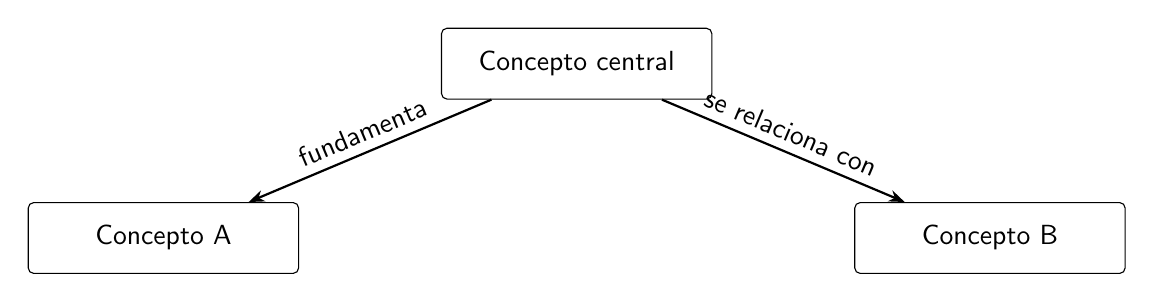
\begin{tikzpicture}[
  concepto/.style={rectangle, draw, rounded corners=2pt,
    align=center, text width=3.2cm, minimum height=0.9cm},
  flecha/.style={-{Stealth[length=2mm]}, thick}
]
\node[concepto] (a) {Concepto central};
\node[concepto, below left=1.3cm and 1.8cm of a] (b) {Concepto A};
\node[concepto, below right=1.3cm and 1.8cm of a] (c) {Concepto B};
\draw[flecha] (a) -- node[above, sloped]{fundamenta} (b);
\draw[flecha] (a) -- node[above, sloped]{se relaciona con} (c);
\end{tikzpicture}
\caption{Mapa conceptual de [tema]}
\end{figure}
\end{verbatim}

\subsubsection*{Línea de tiempo}

\begin{verbatim}
\begin{figure}[H]
\centering
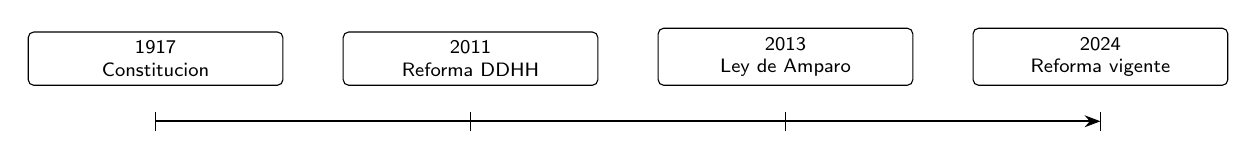
\begin{tikzpicture}[
  evento/.style={rectangle, draw, rounded corners=2pt,
    align=center, text width=3cm, font=\scriptsize},
  eje/.style={-{Stealth[length=2mm]}, thick}
]
\draw[eje] (0,0) -- (12,0);
\foreach \x/\anio/\texto in {
  0/1917/Constitucion,
  4/2011/Reforma DDHH,
  8/2013/Ley de Amparo,
  12/2024/Reforma vigente}
{
  \draw (\x,0.12) -- (\x,-0.12);
  \node[evento, above=0.45cm] at (\x,0) {\anio\\\texto};
}
\end{tikzpicture}
\caption{Linea de tiempo de [tema]}
\end{figure}
\end{verbatim}

\subsubsection*{Diagrama de flujo}

\begin{verbatim}
\begin{figure}[H]
\centering
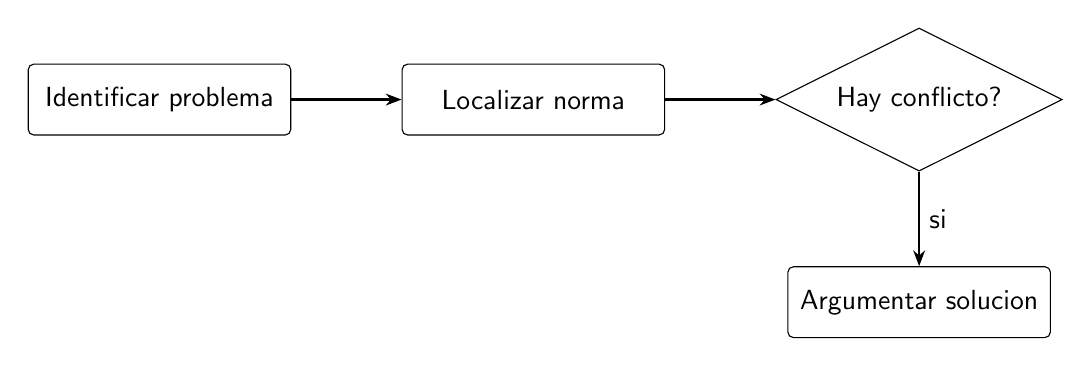
\begin{tikzpicture}[
  paso/.style={rectangle, draw, rounded corners=2pt,
    align=center, text width=3.1cm, minimum height=0.9cm},
  decision/.style={diamond, draw, aspect=2, align=center,
    text width=2.8cm, inner sep=1pt},
  flecha/.style={-{Stealth[length=2mm]}, thick}
]
\node[paso] (inicio) {Identificar problema};
\node[paso, right=1.4cm of inicio] (norma) {Localizar norma};
\node[decision, right=1.4cm of norma] (decision) {Hay conflicto?};
\node[paso, below=1.2cm of decision] (analisis) {Argumentar solucion};
\draw[flecha] (inicio) -- (norma);
\draw[flecha] (norma) -- (decision);
\draw[flecha] (decision) -- node[right]{si} (analisis);
\end{tikzpicture}
\caption{Diagrama de flujo de [proceso]}
\end{figure}
\end{verbatim}

\subsection{Cierre operativo}

La elección de una técnica no debe ser decorativa. Si la actividad pide un producto, la técnica funciona como una herramienta de análisis. El criterio de calidad es que el producto permita ver una decisión intelectual: qué se seleccionó, cómo se organizó, qué relación se construyó y qué postura se puede defender a partir de esa organización.


% ==============================================================================
% REFERENCIAS
% Reglas:
% - Toda fuente citada en el texto debe estar en el .bib.
% - Toda referencia en el .bib debe estar citada en el texto final; quitar
%   fuentes que no se usaron.
% - Toda cita debe tener clave correcta y coincidir con autor/anio visible.
% - Usar fuentes de la planeacion y, si se complementa, que sean confiables.
% - En el cuerpo: \citep{clave}; no usar solo URLs sueltas.
% - Si se trabaja con PDF local, registrar datos bibliograficos completos:
%   autor, anio, titulo, editorial/institucion y URL/DOI si existe.
% - Si la fuente no tiene fecha, usar s. f. con cuidado y preferir confirmar los
%   datos en la portada o ficha bibliografica del documento.
% ==============================================================================
\bibliography{FilosofiaDerechoAct2}

% FIN DEL DOCUMENTO
\end{document}
